\section{Introduction}

\begin{frame}{Introduction}
  \begin{block}{Bérenger Ossété Gombé}
    \begin{itemize}
    \item Bac scientifique en 2013
    \item Maîtrise en informatique (génie logiciel) en 2017
    \item Reconversion web chez Openclassrooms depuis janvier 2022
    \end{itemize}
  \end{block}
\end{frame}

\begin{frame}{Créez une API sécurisée RESTful en utilisant Django REST}
  \begin{block}{Projet 10: parcours python}
    \begin{itemize}
    \item Documenter une application
    \item Créer une API RESTful
    \item Sécuriser une API (OWASP et RGPD)
    \end{itemize}
  \end{block}
\end{frame}

\begin{frame}{Contexte du projet}
  \begin{center}
    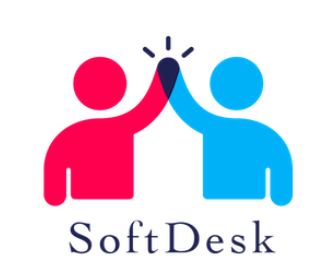
\includegraphics[scale=0.3]{images/logo.png}
  \end{center}
  
  \begin{block}{SoftDesk}
    \begin{itemize}
    \item Société d'édition de logiciels.
    \item Veut développez un \textbf{système de suivi de problèmes}.
    \item Nous sommes ingénieur \textit{backend} sur cette
      application.
    \end{itemize}
  \end{block}
\end{frame}
